
%%%%%%%%%%%%%%%%%%%%%%%%%%%%%%%%%%%%%%%%%%%%%%%
%%%%%   聴覚に関する背景知識と感情音声知覚  %%%%%
%%%%%%%%%%%%%%%%%%%%%%%%%%%%%%%%%%%%%%%%%%%%%%%
\newpage
\chapter{聴覚に関する背景知識と感情音声知覚}
\label{chap:RelatedResearch}

この章では
まず、主に文献\cite{ogushi2019Book, furukawa2021chokaku}を引用して、聴覚に関する基本的な知識や聴覚系における情報分析機能とそのモデル化について述べる。
次に、難聴の種類や高齢者の聴覚特性、模擬難聴処理について説明する。
そして、心理学における感情分類について説明し、これまでに行われてきた感情音声認識実験とその課題について述べる。


%--------------
\section{聴覚末梢系の概要}
\label{sec:Auditory}
%--------------
%参考 山本さん修論 
ヒトの耳は、外耳、中耳、内耳の3つの部分から構成され、聴神経を経て脳へとつながっている。
その様子を図\ref{fig:Hearingsystem}に示す。
耳に到来した音は、耳介の複雑な構造による反射音・直接音の干渉のため、音のスペクトルに変化が生じる。
このスペクトル変化は、音源の空間的位置に依存し、聴空間知覚、特にどの方向から音が聞こえているかという上下・前後方向の音源定位の知覚に重要な役割を果たす。
外耳道を経た音は鼓膜を振動させ、ツチ骨、キヌタ骨、アブミ骨と呼ばれる3つの耳小骨の連鎖を通じて内耳へと伝えられる。
内耳では、主に周波数分析が行われ、数10Hzから20kHzの音が各周波数に対応し、聴神経発火に変換される。
左右の内耳の聴神経から発せられた信号は、一部交差しながら数カ所の中継点を経て、最終的に大脳皮質に達する。
音の音色などの知覚は、大脳皮質の聴覚野によって行われる。

% ---------------------------------------
\begin{figure}[htbp]
    \vspace{40pt}
    \centering
    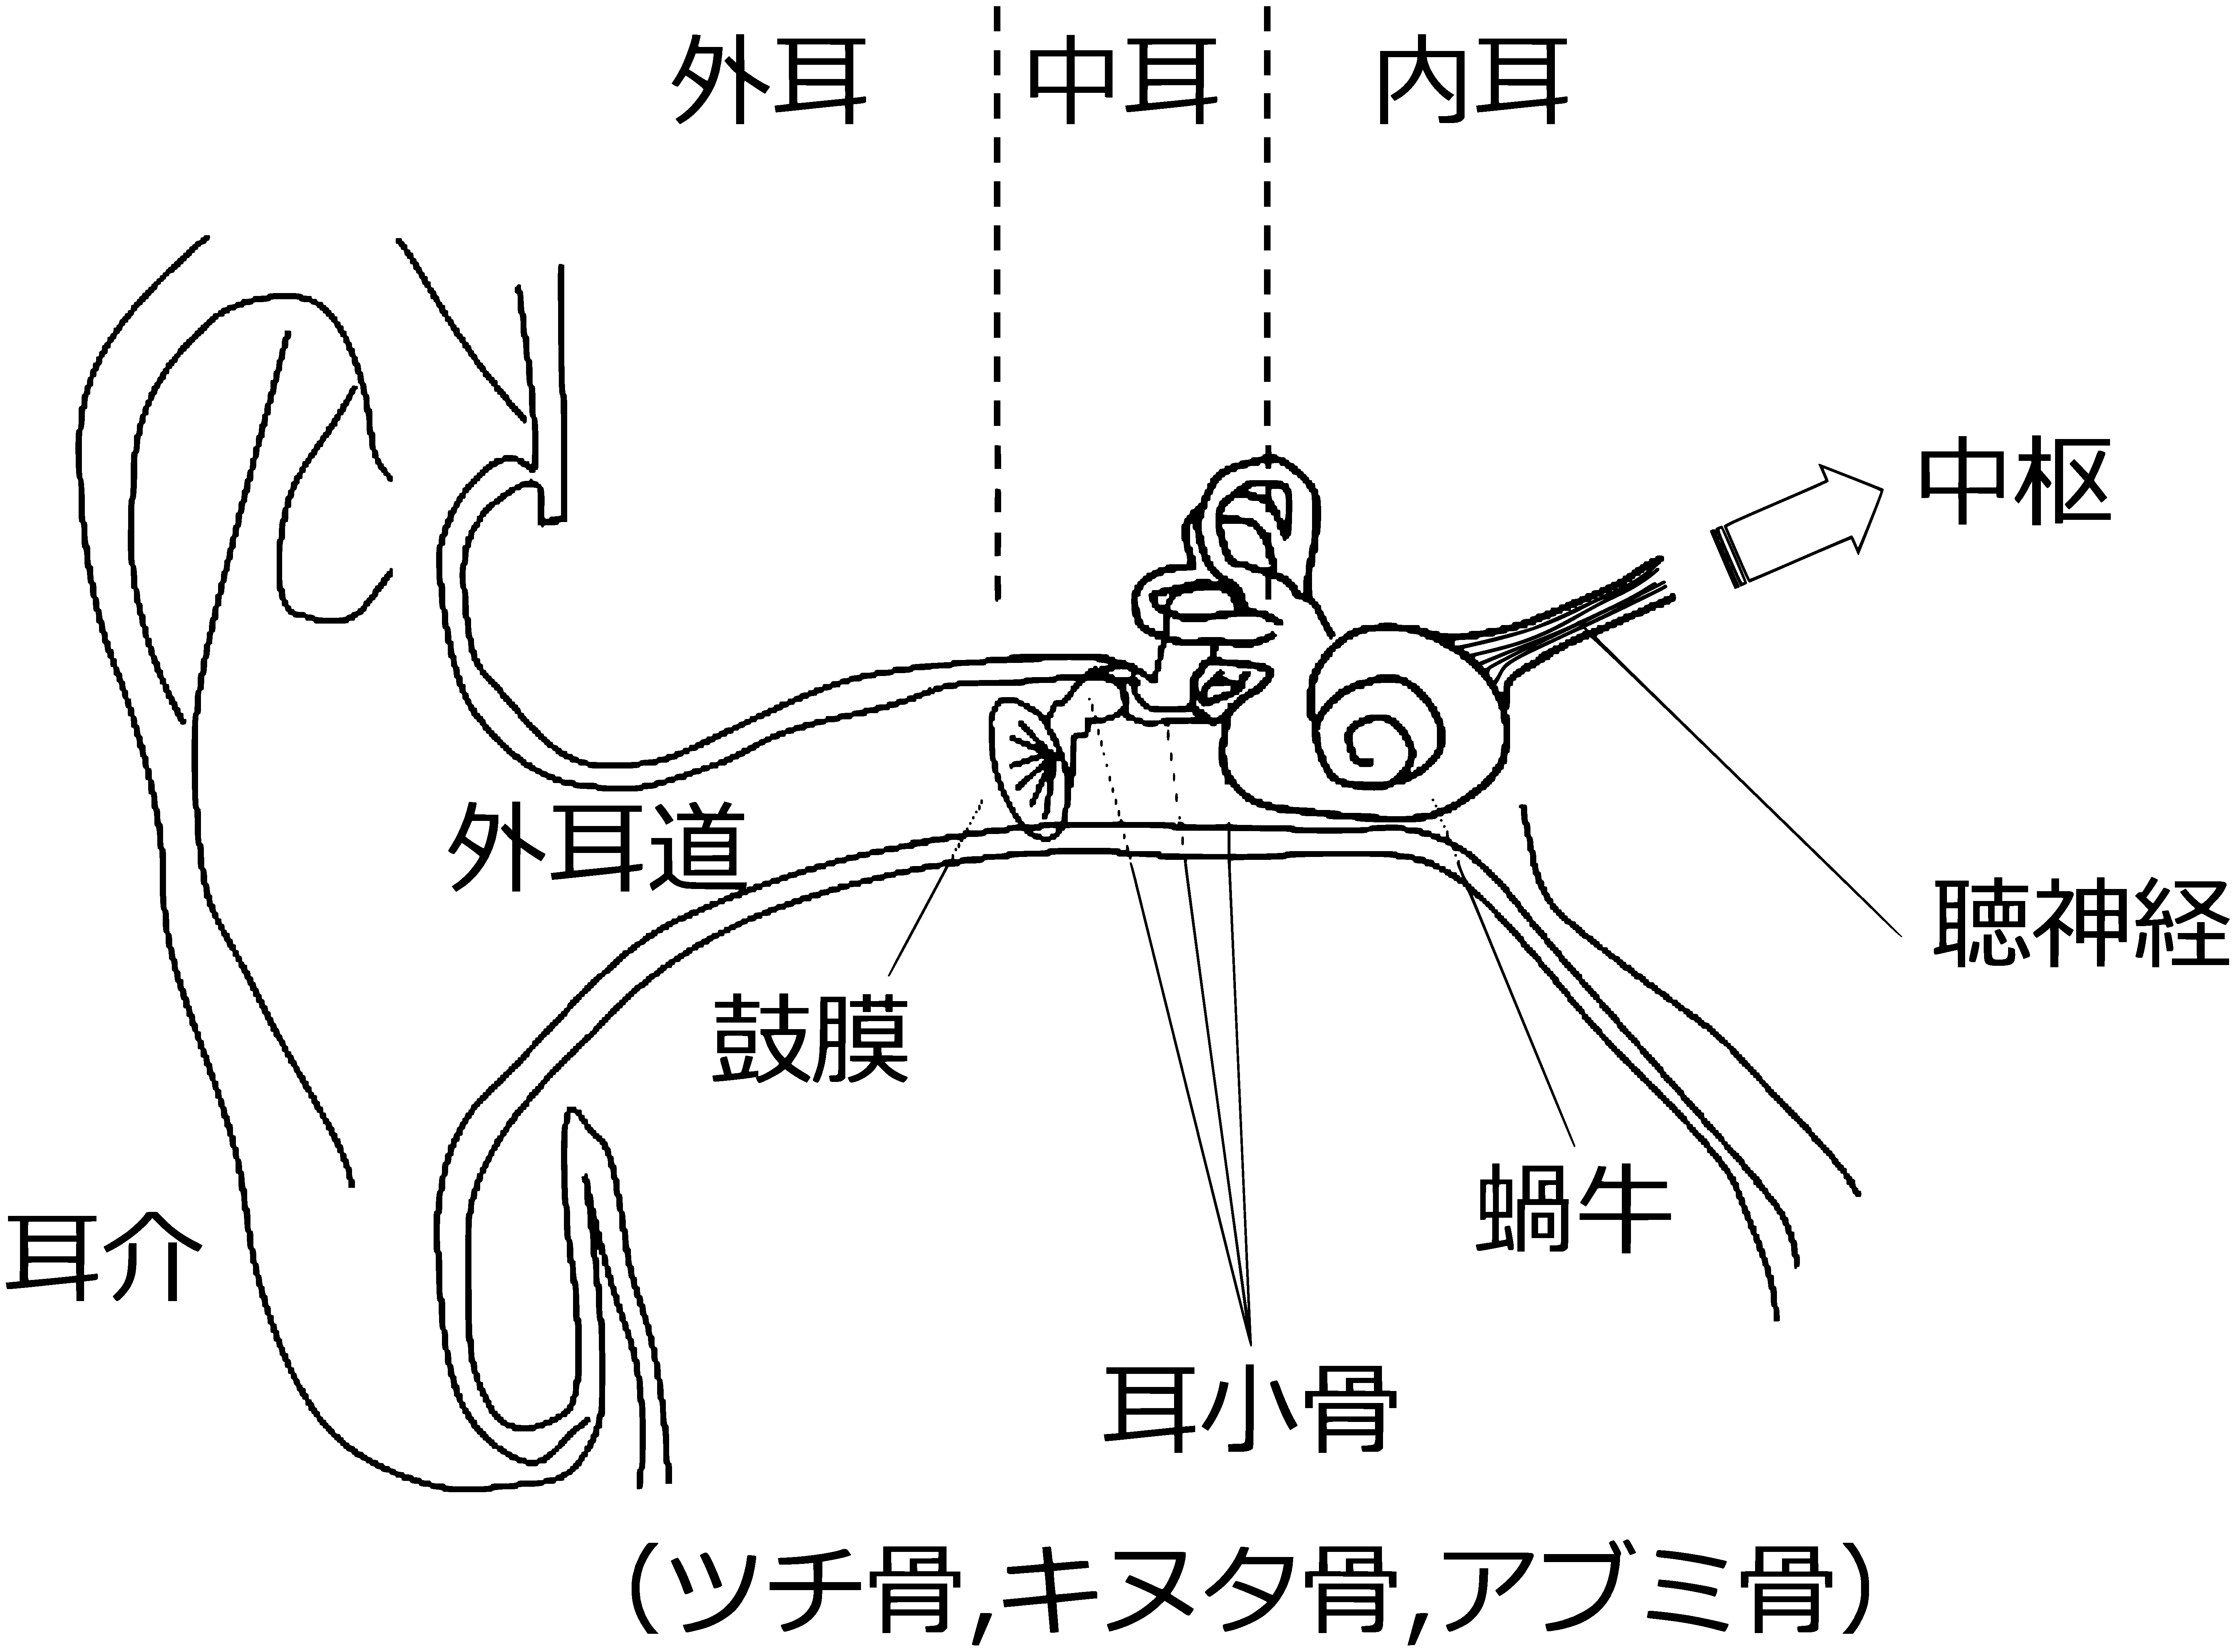
\includegraphics[width=0.6\hsize]{Figure/RelatedResearch/furukawa2017auditory.eps}
    \caption{聴覚末梢系の概観。文献\cite{furukawa2017chokaku}の図1より引用。}
    \label{fig:Hearingsystem}
\end{figure}
% --------------------------------------------


% ==============================
\section{周波数分析機能}
% \label{sec:peripheral}
% ==============================

% ------------------------------
\subsection{聴覚フィルタ}
% \label{sec:auditory filter}
% ------------------------------
前節で述べたように、蝸牛に到達した音は、基底膜が機械的に振動することで周波数分析された後に聴神経発火へ変換される。
この基底膜振動に由来する周波数分析あるいは周波数選択性を、心理物理学において聴覚フィルタ(auditory filter)と呼ぶ。

基底膜の機械振動が最大となる場所は、入力された音の周波数によって変化する。
この様子は、信号処理の観点から、中心周波数と帯域幅が異なる多数の聴覚フィルタが並んでいると考えられ、
このフィルタ群全体を聴覚フィルタバンク(auditory filterbank)と呼ぶ。
蝸牛頂側には低周波数域に対応する聴覚フィルタ、耳小骨側では高い周波数に対応する聴覚フィルタが並んでいる。

% ---------------------------------------
\begin{figure}[h]
  \vspace{20pt}
  \centering
  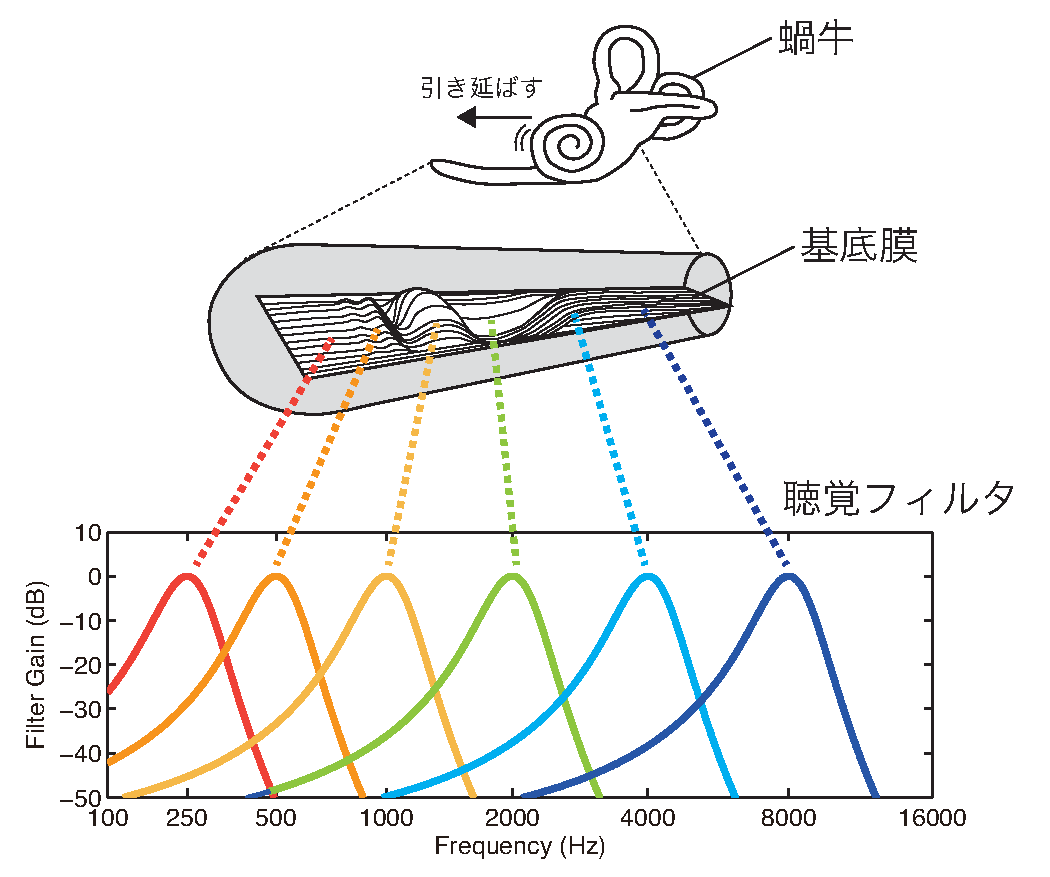
\includegraphics[width=0.6\hsize]{Figure/RelatedResearch/KiteimakuAudFilter.eps}
  \caption{聴覚フィルタの模式図。蝸牛を引き延ばした図(中段)では、基底膜の振動の様子を表している。
            入力音の周波数によって基底膜上の振動する場所が異なる。このような内耳での周波数分析は、
            聴覚フィルタ(下段)が並んでいる形で定式化できる。文献\cite{higashiyama2020WHIS}の図1.6より引用。}
  \label{fig:BasilarMembrane}
\end{figure}
% --------------------------------------------

% ------------------------------
\subsubsection{振幅周波数特性}
% ------------------------------
図\ref{fig:Basic_FilterBank}に6つの中心周波数をもつ聴覚フィルタの振幅周波数特性の例を示す。
横軸は周波数、縦軸はフィルタの利得である。
心理物理学では、このような振幅周波数特性の2乗のパワースペクトルのことをフィルタ形状と呼ぶ。
% ただし横軸は、対数周波数尺度に近い非線形周波数軸(後述の$\mathrm{ERB_{N}}$番号軸)となっている。
図\ref{fig:Basic_FilterBank}より入力された音圧が一定の場合、聴覚フィルタは中心周波数に関わらず同じような形状をもつことがわかる。
また、その周波数特性は中心周波数に対して非対称である。
さらに、外界の音圧や音環境によって変化する非線形フィルタとなっている。

聴覚フィルタの特性は個人ごとに異なり、特に高齢者や難聴者の場合は標準的な特性から大きくばらつく。
そのため、個人の特性に合わせたモデル化が必要とされている。

% ------------------------------
\subsubsection{聴覚フィルタの帯域幅}
% ------------------------------
ここで、健聴者の聴覚フィルタの中心周波数\textcolor{red}{$F$[Hz]}と帯域幅は、
おおよそ以下の関係であることが心理物理学測定から知られている\cite{moore2013introduction}。

\begin{equation}
	\mathrm{ERB_N} = 24.7 \times\bigl(\frac{4.37F}{1000} + 1\bigr)
    \label{eq:ERB}
\end{equation}

等価矩形帯域幅(equivalent rectangular bandwidth; $\mathrm{ERB_N}$)とは、
図\ref{fig:ERB}のようにある中心周波数\textcolor{red}{$F$[Hz]}の聴覚フィルタのパワースペクトル上での面積を、
聴覚フィルタの最大利得と等しい高さをもつ長方形(矩形)で表現した場合の帯域幅(底辺)である。
この等価矩形帯域幅自体は、任意のフィルタ形状で計算することができる。
この中心周波数によって変わる帯域幅のフィルタが、同一形状で等間隔に並ぶように$\mathrm{ERB_N}$番号($\mathrm{ERB_N}$ number)が定義されている。%(単位: Cam)。
\textcolor{red}{
    単位はCam であり、何番目の聴覚フィルタであるかを指す尺度とみることもできる\cite{unoki2021Method}。
    この単位は、提唱者であるMooreらの研究所の所在地であるCambridgeにちなんでつけられた\cite{hartmann2004Signal}。 
}

\begin{equation}
    \mathrm{ERB_N \ number} = 21.4 \log_{10} \bigl(\frac{4.37F}{1000} + 1\bigr)
\end{equation}

% ---------------------------------------
\begin{figure}[h]
    % ---------------------------------------
    \begin{minipage}[c]{0.45\hsize}
    \vspace{50pt}
    \centering
    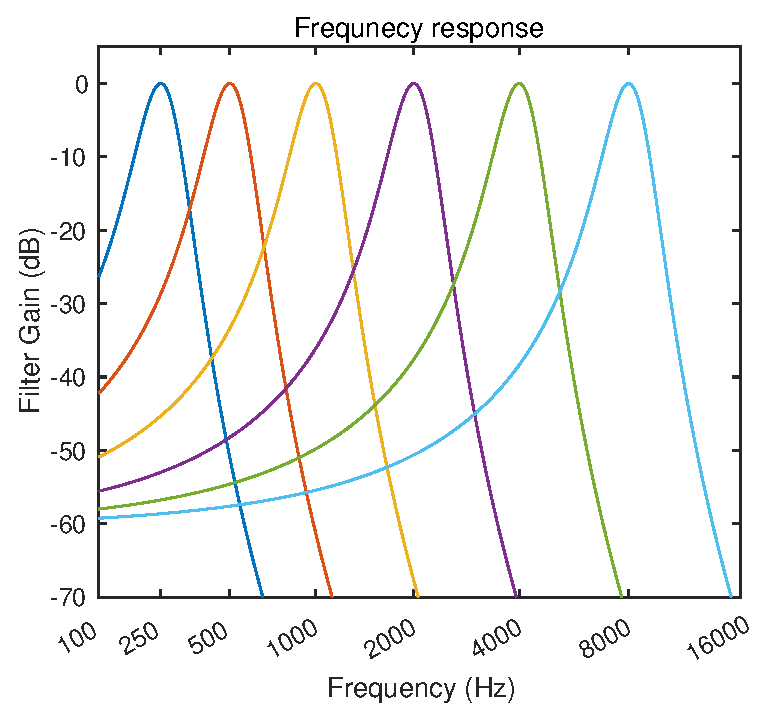
\includegraphics[width=\hsize]{Figure/RelatedResearch/DemoAF_Basic_FilterBank.eps}
    \caption{聴覚フィルタの周波数特性の例。一定音圧の場合で、中心周波数が250, 500, 1000, 2000, 4000, 8000Hzの6種類の聴覚フィルタを示す。文献\cite{irino2010hajimete}の図1より引用。}
    \label{fig:Basic_FilterBank}
    \end{minipage}
    % ---------------------------------------
    \hspace{0.1\hsize}
    \begin{minipage}[c]{0.45\hsize}
    \vspace{50pt}
    \centering
    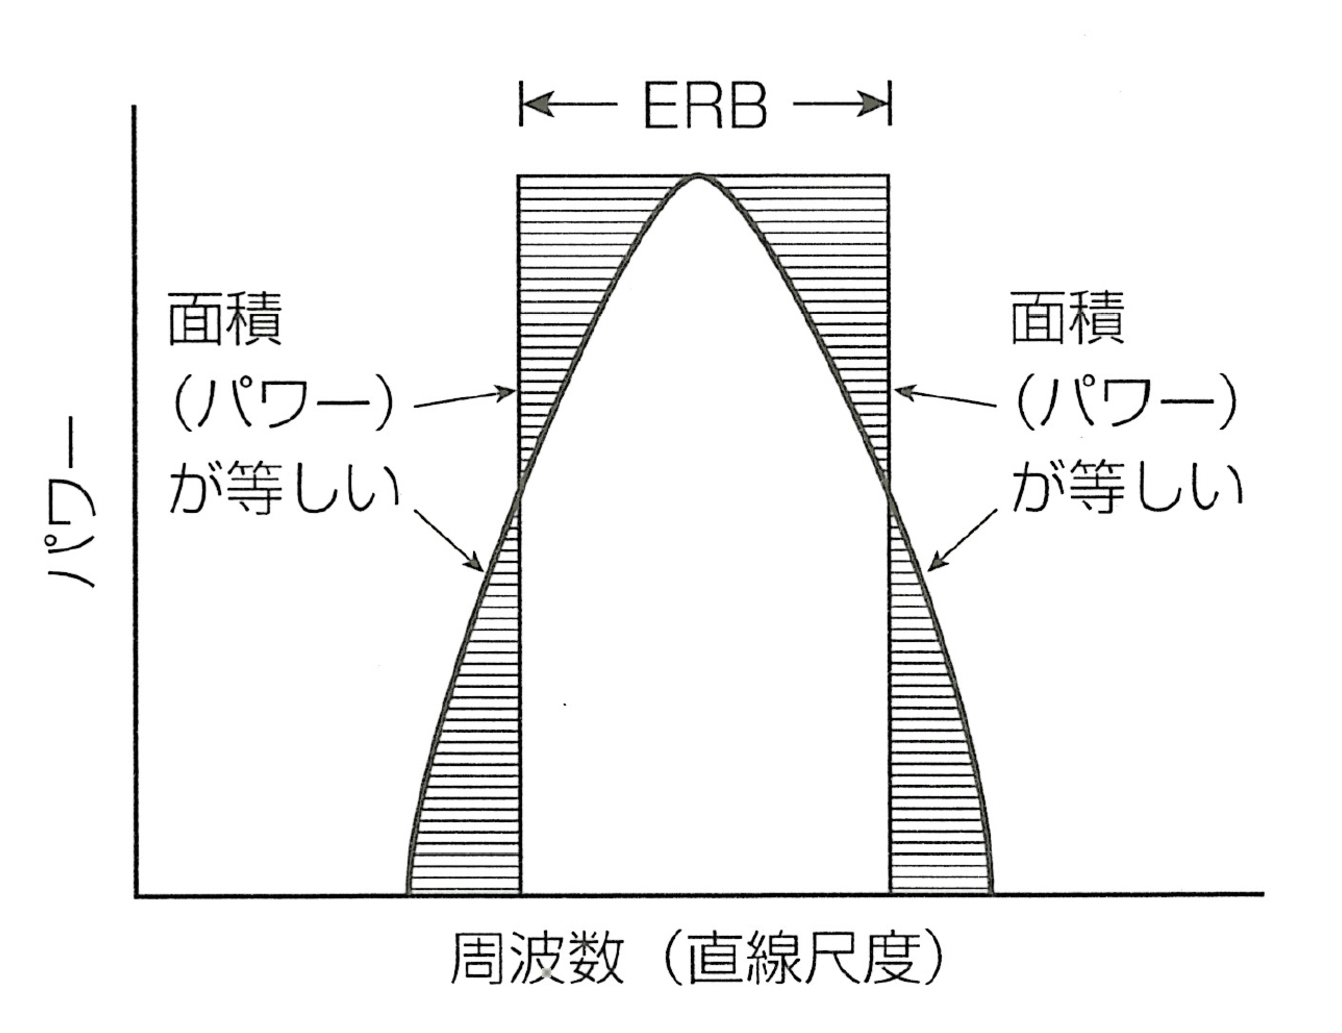
\includegraphics[width=1.08\hsize]{Figure/RelatedResearch/Ogushi2019ERB.eps}
    \caption{等価矩形帯域幅(ERB)。曲線はある中心周波数の聴覚フィルタを示す。文献\cite{ogushi2019Book}の図4-15より引用。}
    \label{fig:ERB}
    \end{minipage}
\end{figure}
% --------------------------------------------


\newpage
% ------------------------------
\subsection{音圧依存性}
\label{sec:FilterLevelDepend}
% ------------------------------
実際の聴覚フィルタは、外界の音環境や音圧に依存して、その形状や利得が変化する非線形の時変フィルタである。
音圧に対するフィルタ形状と利得の変化の例を図\ref{fig:Basic_FilterLevelDepend}に示す。
入力音の音圧が30dBのとき、中心周波数における利得は最も大きく、音圧が上昇するとともに利得が減少することがわかる。
さらに、フィルタの帯域幅も音圧上昇と共にやや広くなる傾向があることもわかる。
    
% ------------------------------
\subsection{圧縮特性}
\label{sec:IOfunc}
% ------------------------------
図\ref{fig:Basic_IOfunc}は、図\ref{fig:Basic_FilterLevelDepend}で示した聴覚フィルタの特性(音圧依存性)から計算される、
フィルタの入力音圧と出力音圧の関係を示すグラフである。
破線で示された増加率が1\,dB/\,dB(1:1)の線形関係を表している。
実線で表された健聴者の聴覚フィルタの入出力特性は、破線に比べて緩やかな傾きであり、中程度の音圧域で約0.2$\sim$0.3\,dB/\,dBの増加率になると推定されている。
このような、入力音圧が小さい場合利得が大きく、入力音圧が上昇するにしたがって利得が小さくなる聴覚フィルタの特性を圧縮特性と呼ぶ。

% ---------------------------------------
\begin{figure}[h]
    % ---------------------------------------
    \begin{minipage}[t]{0.5\hsize}
        \vspace{50pt}
        \centering
        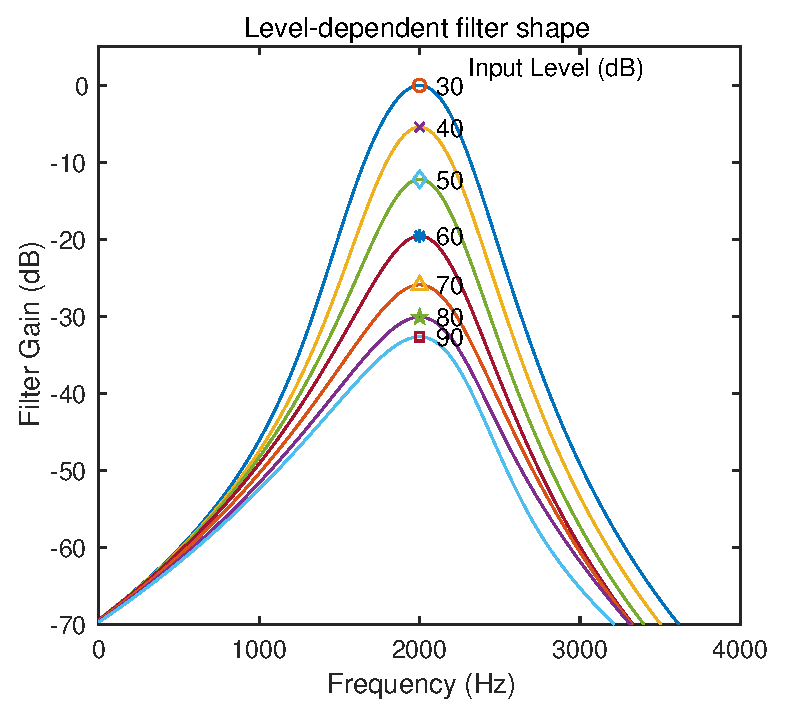
\includegraphics[width=\linewidth]{Figure/RelatedResearch/DemoAF_Basic_FilterLevelDepend.eps}
        \subcaption{音圧依存性}
        \label{fig:Basic_FilterLevelDepend}
    \end{minipage}
    % ---------------------------------------
    \begin{minipage}[t]{0.5\hsize}
        \vspace{50pt}
        \centering
        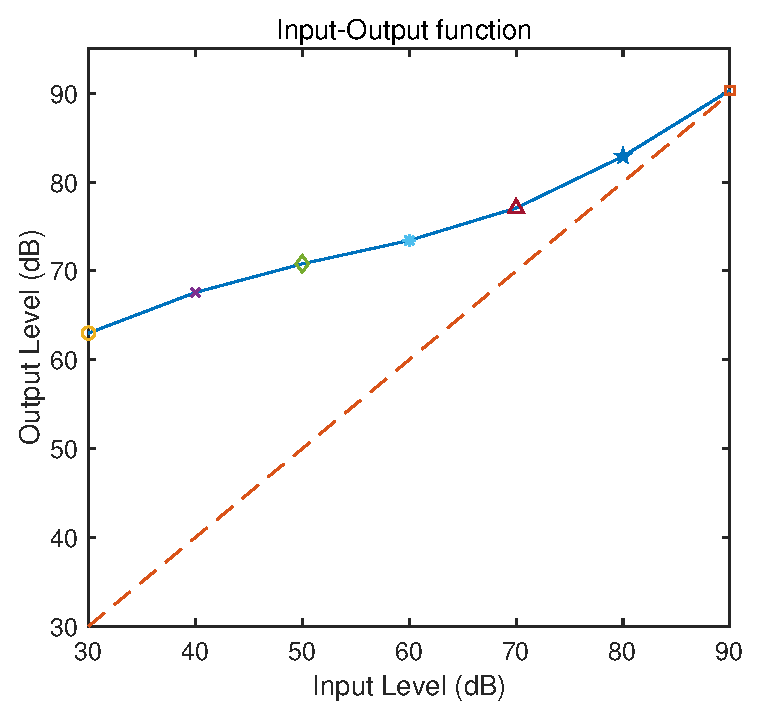
\includegraphics[width=0.96\linewidth]{Figure/RelatedResearch/DemoAF_Basic_IOfunc.eps}
        \subcaption{入出力特性}
        \label{fig:Basic_IOfunc}
    \end{minipage}
    \label{compression}
    % ------------------------------------------
    \caption{聴覚フィルタの音圧依存性(a)と入出力特性(b)の例。図中の記号と色は対応している。
            \textcolor{red}{(a)音圧が低いとフィルタの利得が大きく、音圧上昇とともに利得は減少する。一番小さい入力音圧レベル(30dB)のときの利得の最大値が0dBになるように、正規化を行なっている。
            (b)図(a)の入力音圧に対する最大利得の値を用いて、対応する出力音圧を計算し、入力90dBに対して出力90dBとなるようにレベルを調整している。}
              文献\cite{yamamoto2023GESI}の図2.3,図2.4より引用。}
\end{figure}
% --------------------------------------------

\newpage



% フィルタ形状の推定〜ガンマチャープフィルタ は略

\clearpage
 % ==============================
\section{時間分析機能}
% \label{sec:peripheral}
% ==============================
音声や音楽など、日常生活のほぼ全ての音は時間的に変動している。そして、その時間変動のパターンの中から、聴覚系は音源や環境に関する情報を取り出している。
時間変動に含まれる情報は、末梢系の周波数分析を経た中枢系において行われている。具体的なメカニズムに関しては、十分に理解が進んでいるとは言えず、あくまで暫定的な仮説に基づいたアプローチが広く用いられている。

聴覚フィルタの出力波形は振幅包絡(変調波)と時間微細構造(temporal fine structure; TFS; 搬送波) のふたつの成分に分類して考えられる。
一般に、音声の時間微細構造をなくして、振幅包絡情報だけで音声知覚ができることが示されている。
ピッチ知覚や両耳間時間差に基づいた音源の分離(たとえば音源定位)においては、TFSの情報が重要である。

% TMTF
時間分解能の劣化度合いを表す指標として、Gap検知閾(gap detection threshold; GDT)と時間変調伝達関数(temporal modulation transfer function; TMTF)等がある。
TMTFは、振幅包絡情報としての変調周波数と変調度の閾値を測定できるため、補聴器への応用や難聴者の聴覚指標として重要であると考えられている。
このTMTFの測定には、従来手法であれば約20 $\sim$ 40分を要し、臨床への応用が困難とされてきた。
近年では、その解決策として短時間で測定可能な2点法による測定が提案されている\cite{morimoto2019Two-PointTMTF}。
TMTFは、通常、7変調周波数における変調度の閾値を測定し、それら変調度の閾値を1次のバタワースフィルタで最小二乗近似を行い、peak sensitivity ($L_{ps}$)と 3dB cutoff frequency ($f_{cutoff}$)を算出する。
2点法では、以下の2点の測定結果のみから$L_{ps}$と$f_{cutoff}$を算出する。
1つが、変調周波数8Hzの振幅変調音において、知覚可能な変調度[dB, 20log(m)]の閾値$L{\alpha}$である。
もう1つが、閾値$L_{\alpha}$を2で除した値 ($L_{\alpha}$/2)を変調度とした振幅変調音において、知覚可能な変調周波数[Hz]の閾値$f_{\beta}$である。
このような手法で、測定時間を約10分に短縮した。

% ---------------------------------------
\begin{figure}[h]
    % ---------------------------------------
    \begin{minipage}[b]{0.5\hsize}
        \vspace{50pt}
        \centering
        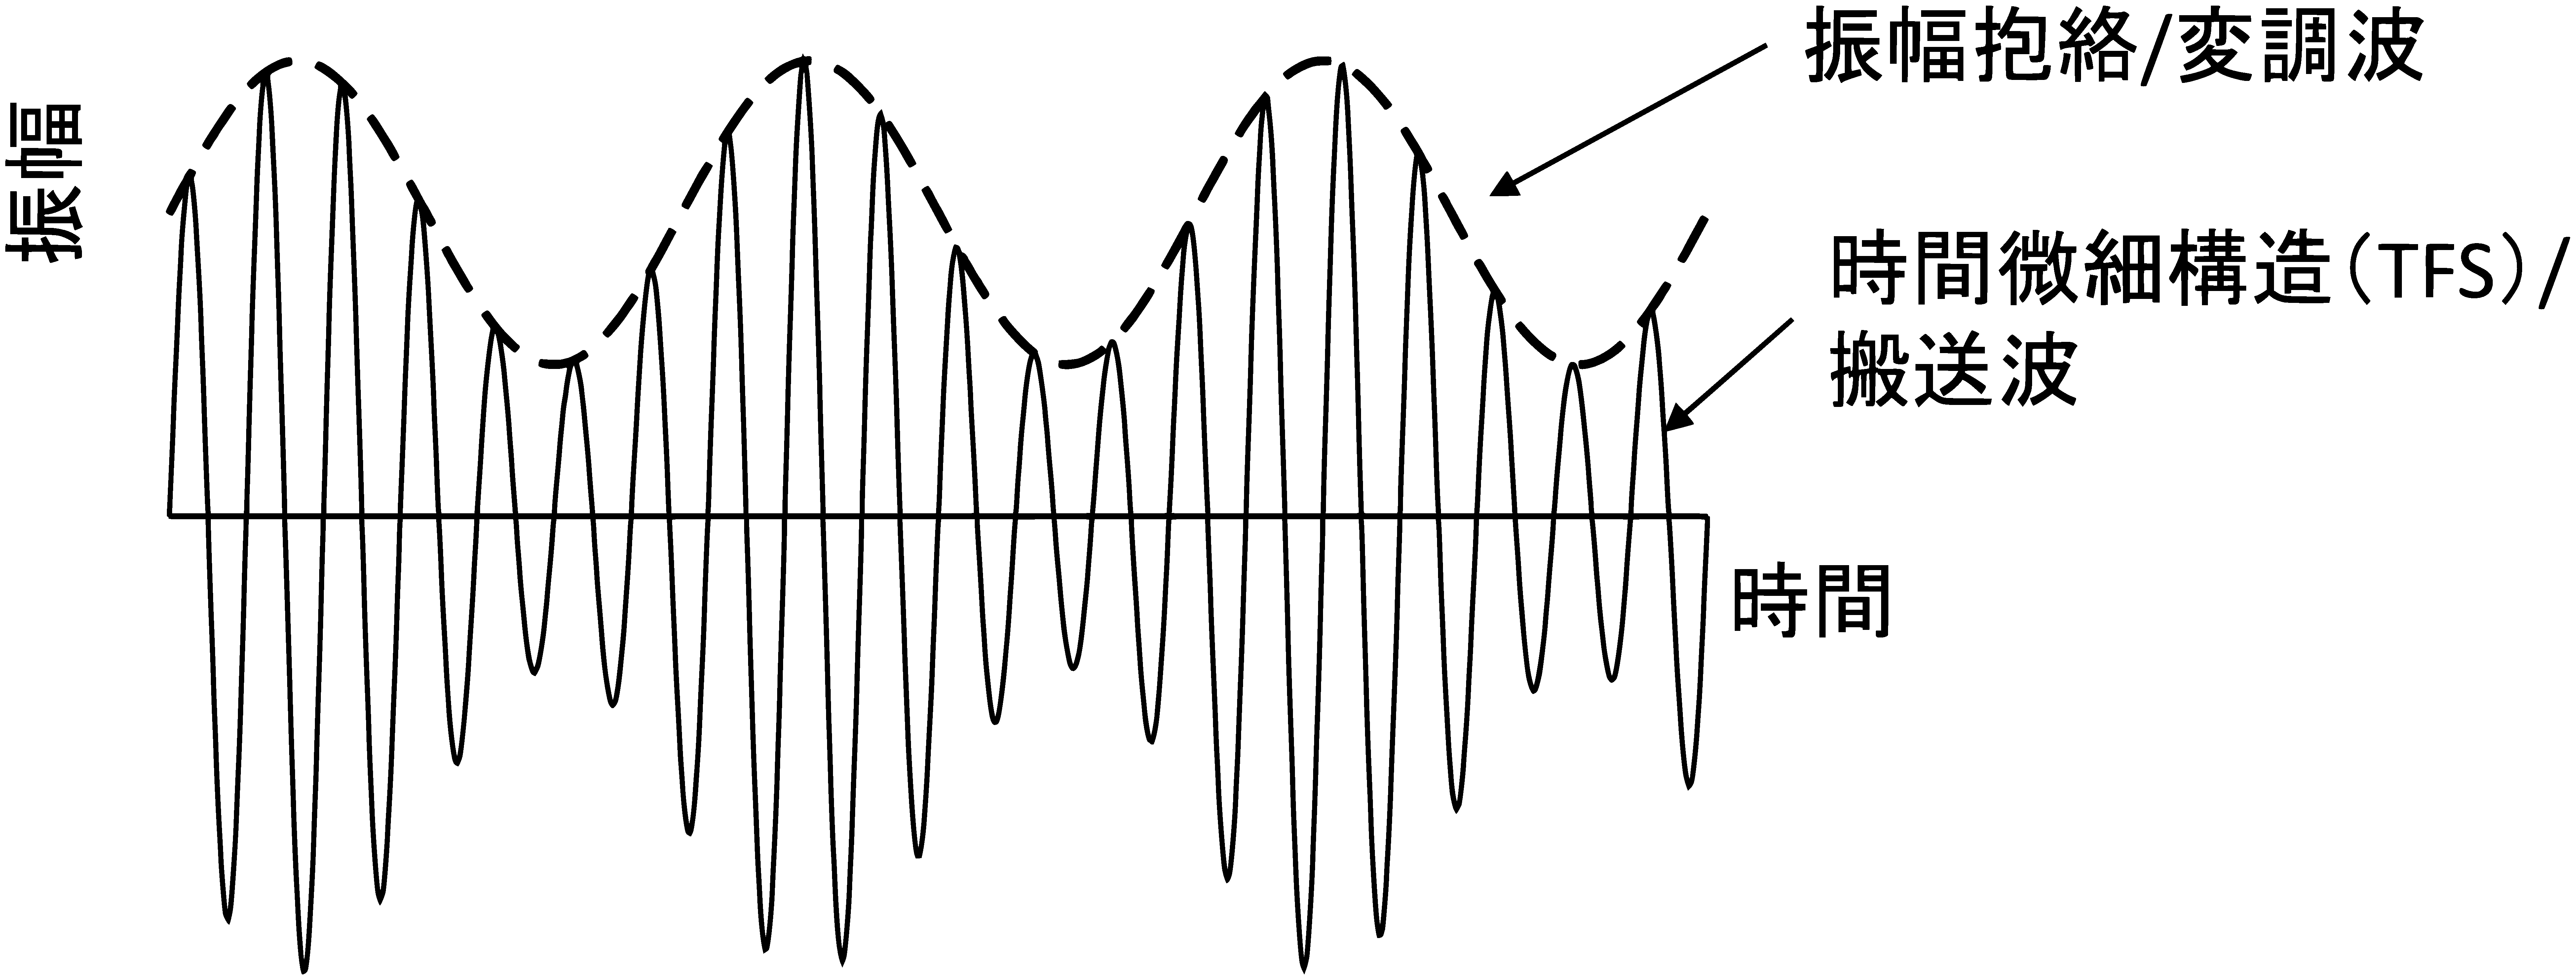
\includegraphics[width=1.07\hsize]{Figure/RelatedResearch/furukawa2016time.eps}
        \caption{振幅包絡と時間微細構造。文献\cite{furukawa2016time}の図1より引用。}
        \label{fig:TFS}
    \end{minipage}
    % ---------------------------------------
    \hspace{0.05\hsize}
    \begin{minipage}[b]{0.45\hsize}
        \vspace{50pt}
        \centering
        \includegraphics[width=\hsize]{Figure/RelatedResearch/FigTMTF.eps}
        \caption{2点法で使用される測定パラメタ。文献\cite{morimoto2019Two-PointTMTF}の図2より引用。}
        \label{fig:TMTF}
    \end{minipage}
    
    % ------------------------------------------
    % \caption{}
\end{figure}
% --------------------------------------------
% % ---------------------------------------
% \begin{figure}[h]
%     \vspace{40pt}
%     \hspace{20pt}
%     \centering
%     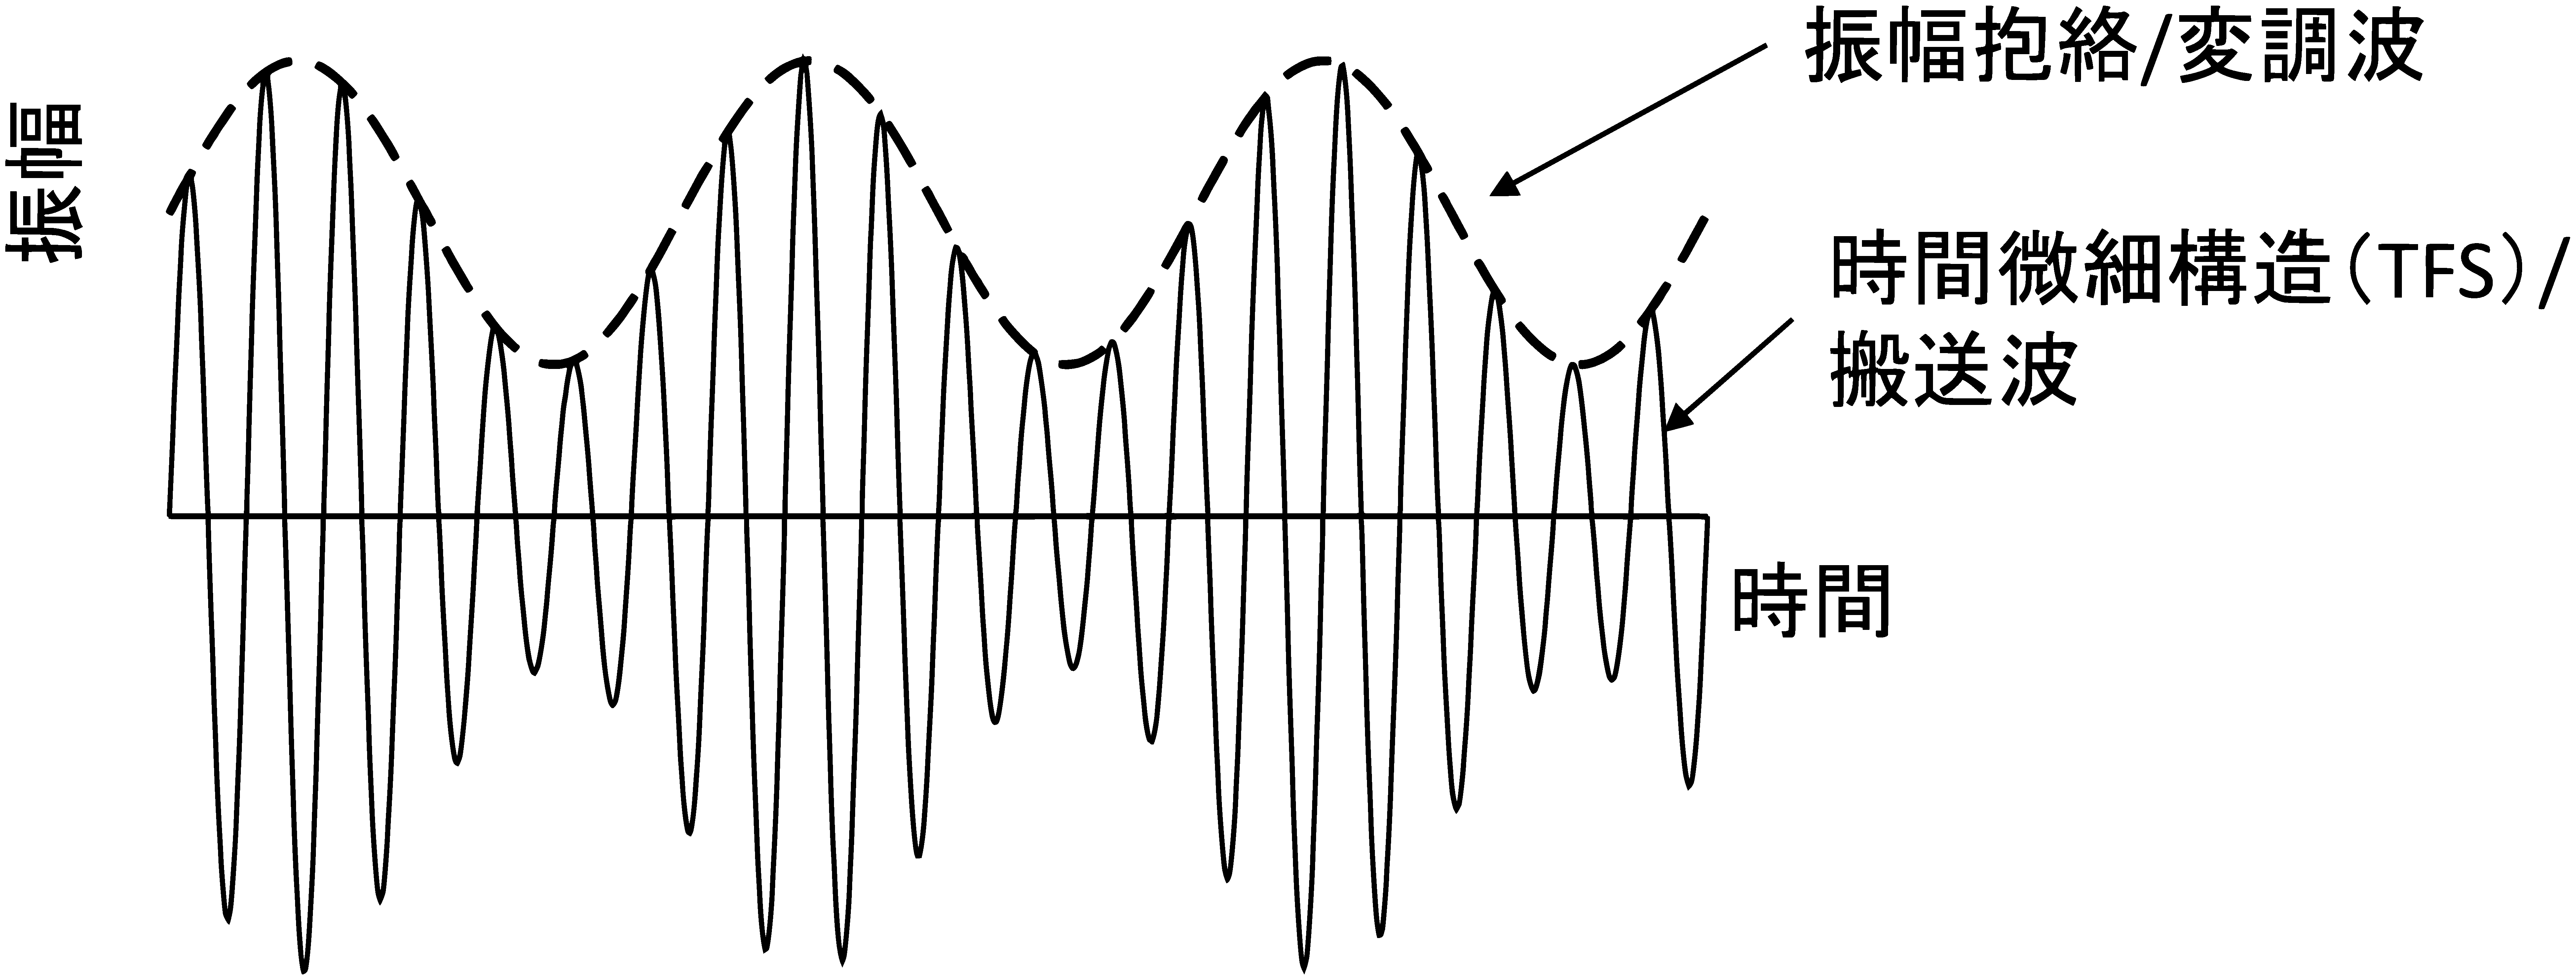
\includegraphics[width=0.8\hsize]{Figure/RelatedResearch/furukawa2016time.eps}
%     \caption{振幅包絡と時間微細構造。文献\cite{furukawa2016time}の図1より引用。}
% \end{figure}
% % --------------------------------------------

% 変調フィルタバンク は略


\clearpage
% ==============================
\section{高齢者の聴覚特性}
% ==============================
高齢になると多くの人が加齢性難聴に悩む。
加齢性難聴の最も深刻な問題が、音声聴取が困難になること、つまり相手の声は聞こえても何を言っているのか理解できない状況である。
この状況がひどくなり、音声による対人コミュニケーションが困難になると社会的生活活動に支障が生じ、社会的孤立、うつ、自己評価の低下につながる危険性がある。

% ------------------------------
\subsubsection{難聴の種類}
% ------------------------------
難聴には、聴覚機能が損なわれた原因によって分類される。
それぞれの特徴を以下にまとめる。

\begin{itemize}
\item \textbf{伝音性難聴 (conductive hearing loss)}\\
 外耳および中耳に機械的障害が生じることにより発生する。
 鼓膜や中耳の耳小骨(ツチ骨、キヌタ骨、アブミ骨)の損傷が一般的である。
 障害の部位と程度により、聞き取りにくい周波数や聴力レベルは多様であるが、純音聴力検査で気導聴力が70dBHLを超えることはない。
 伝音機能が完全に失われても、エネルギーの大きな音は骨導音として内耳に伝達するためである。
\item \textbf{感音性難聴 (sensorineural hearing loss)}\\
 内耳に障害が生じることにより発生する。
 蝸牛の有毛細胞や聴神経の障害による内耳性難聴(cochler hearing loss)と聴神経系に障害を生じる後迷路難聴(retrocochler hearing loss)がある。
\end{itemize}


% ------------------------------
\subsubsection{加齢性難聴の生理学的要因}
% -----------------------------
加齢性難聴は、末梢系にも中枢系にも要因があると考えられている。
末梢系については大まかに以下の4種類に分類されている\cite{Schuknecht1993presbycusis}。
\begin{itemize}
\item 感覚細胞系:蝸牛内の内有毛細胞・外有毛細胞・支持細胞の損傷
\item 神経細胞系:蝸牛の求心性ニューロンの損傷
\item 代謝系:蝸牛側壁や血管条の萎縮
\item 機械系:基底膜やコルチ器の硬化
\end{itemize}
ただし、これらの要因が混じりあったり、不明な要因による機能低下も存在する。
高齢者に多い高い周波数領域の聴力損失は、蝸牛の有毛細胞の損傷・消失が主な原因となっている。
% ヒトは日常生活において長い間騒音にさらされており、有毛細胞の損傷・消失の大きな原因となっているが、静かな場所で育った動物においても老化の影響があり、有毛細胞は消失していく。



\clearpage
% ------------------------------
\subsubsection{高齢者の純音閾値の周波数特性}
% -----------------------------
さまざまな周波数の純音に対する聴取者の最小可聴閾値(聴覚閾値)の測定は、純音聴力検査(pure tone audiometry)と呼ばれ、
オージオメータ(audio meter)により125, 250, 500, 1000, 2000, 4000, 8000Hzの7つの周波数の純音に対して測定が行われる。
測定結果を図として表したものはオージオグラム(audiogram)という。
若年健聴者の正常聴力閾値を基準(0dB)とし、その値より高くなった閾値のレベルをdBで表現する。
この値を聴力レベル(Hearing level; HL)と呼び、その値が大きいほど聴力が低下していることを意味する。

立木らは、通常の社会生活を営む一般社会人男女約1500人を対象にして聴力レベルを測定した\cite{tuiki2003eldery}。
年代ごとの平均値を表示した例を図\ref{fig:Audiogram}に示す。
この図から、年齢の上昇とともに、全体的に聴力が低下していくが、特に高周波数域の聴力低下の程度が著しくなることがわかる。
さらに、聴力損失は年齢を重ねるほど進行速度が加速される傾向がある。

また、音声聴取に特に重要な 500, 1000, 2000, 4000Hzの4周波数に対して、良い方の耳の聴力レベル(dB)の平均値を代表値(4周波数平均聴力レベル)とし、

\begin{equation}
平均聴力レベル = \frac{HL_{\mathrm(500Hz)} + HL_{\mathrm(1000Hz)} + HL_{\mathrm(2000Hz)} + HL_{\mathrm(4000Hz)}}{4}\\
\end{equation}
の式で計算によって求める。
WHO基準(Prevention of blindness and deafness)では、この平均聴力レベルが25 dB以下であれば正常聴力(健聴者)、26--40 dBであれば軽度難聴、
41--60 dBであれば中等度難聴、61--80 dBであれば高度難聴、81 dBであれば重度難聴と定められている。
% ただし、難聴の基準にはさまざまな種類が存在し、平均聴力レベルの算出には4分法と呼ばれる以下のような方法もある。
% \begin{equation}
% 平均聴力レベル = \frac{HL_{\mathrm(500Hz)} + \bigl(HL_{\mathrm(1000Hz)}\bigr)×2 + HL_{\mathrm(2000Hz)}}{4}\\
% \end{equation}

% なお、本研究では、従来の感情認識実験\cite{christensen2019effects}に基づき、正常聴力(健聴者)を平均聴力レベルが22 dB以下とした。
% % ---------------------------------------
\begin{figure}[h]
    \centering
    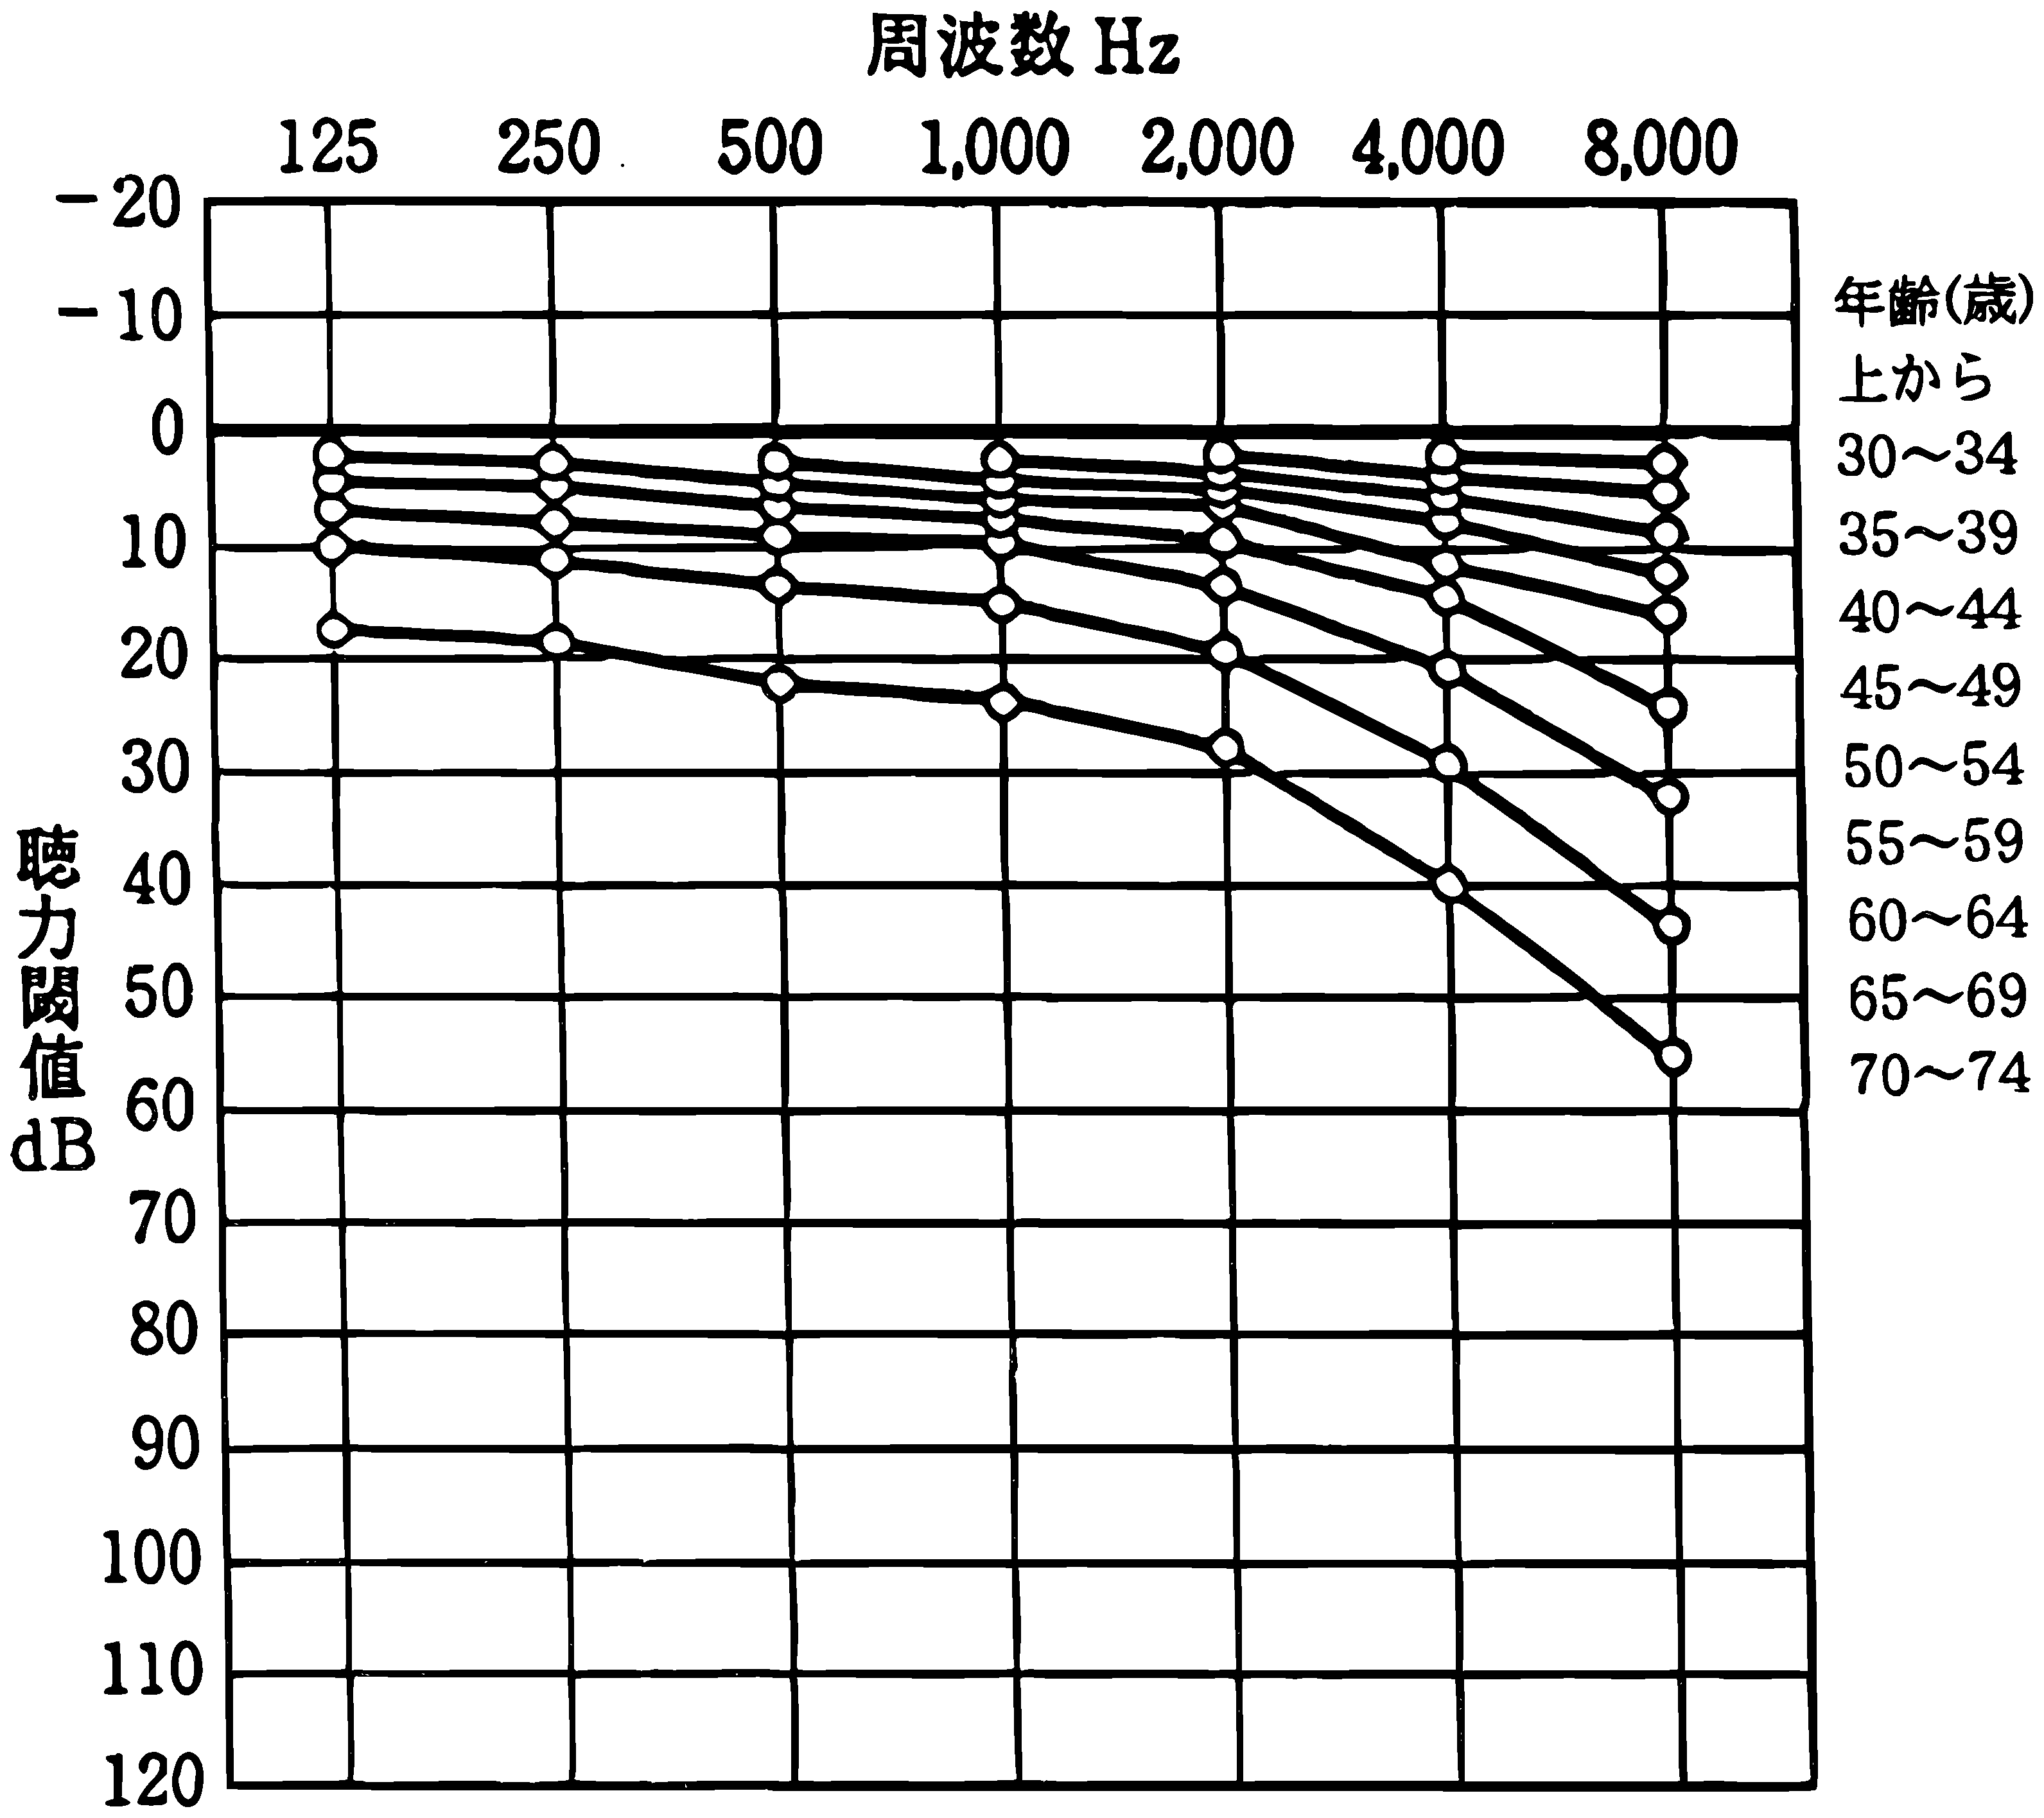
\includegraphics[width=0.6\hsize]{Figure/RelatedResearch/Tsuiki2003Audiogram.eps}
    \caption{年齢別平均オージオグラム(30--74歳, 実測値)。文献\cite{tuiki2003eldery}の図2より引用。}
    \label{fig:Audiogram}
\end{figure}
% % --------------------------------------------



% ------------------------------
\section{模擬難聴システムWHISによる末梢系の機能低下の模擬 \cite{irino2022moginancho,irino2023hearing}}
\label{sec:WHIS}
% ------------------------------ 
% 模擬難聴とは、健聴者が難聴者の聞こえを体験できる技術である。
% 健聴者が難聴者の困難さを体験できると、難聴者への話しかけ方の改善等につながり、
% 体験型学習や言語聴覚士の養成、患者家族との面談において有用となることが期待されている。
% この模擬難聴は聴覚心理実験に応用されている。
% 難聴者を対象とした聴取実験はこれまでも行われてきたが、難聴者ごとに機能低下の度合いや要因には大きなばらつきがある。
% また、加齢性難聴であれば認知機能の高低も影響する。
% さらに、長時間の聴取実験は集中力維持の観点から難しい。
% そこで、聴覚心理実験において、刺激音を模擬難聴システムを通して若年健聴者が聞くことにより
% 「模擬難聴者」として被験してもらう手法が提案された。
% これにより、認知的問題や集中力問題を回避しつつ、末梢系の特性に関して統制が取れ、
% 少人数でも短時間で明確な結果が得られる可能性が期待されている。

模擬難聴処理システムWHISは、永江らによって開発された健聴者が難聴者の聞こえを体験できる技術である\cite{nagae2016WHIS}。
また、近年WHISの新実装版が開発され\cite{irino2023hearing}、様々な聴覚心理実験に応用されている。


% from ASJ解説25 参照日:26Jan2025,  from irino2022moginancho
高齢難聴者の場合、オージオグラム上の高域で聴力レベルが低下する。
これは、聴覚末梢系の蝸牛における外有毛細胞が担う増幅作用の低下と,振内有毛細胞が担う振動を神経発火に変換する機能の低下の両方の影響による。
前者は入力の広いダイナミックレンジに対してレベル依存する能動的な処理とみなせ、後者は受動的な線形に近い処理とみなせる。
オージオグラムは、それぞれの機能低下の割合を示さず、全体的な閾値上昇だけを示す。
ここで、オージオグラム上の聴力レベル$HL_{total}$は、能動的な聴力損失$HL_{act}$と受動的な聴力損失$HL_{pas}$とのdB上での和で表せると仮定する\cite{moore1997model}。

% 聴覚末梢系の蝸牛においては、外有毛細胞が担う増幅作用と、内有毛細胞が担う振動を神経発火に変換する機能がある。
% 蝸牛以降の機能低下の要因もありうるが、加齢性難聴に限定すれば、ある程度良い近似となっていると考えられる。
WHISでは、この図式を反映できる圧縮型ガンマチャープ聴覚フィルタ\cite{irino2001compressive,irino2006dynamic}を用いている。

% 後者に蝸牛以降の若干の受動的なレベル低下の要因も含めて考えても良いかもしれない。

図\ref{fig:EP_HI=NH+WHIS}に、上記の聴覚モデルを基本とした、模擬難聴処理の概念図を示す。
図\ref{fig:EP_HI=NH+WHIS}(a)に、模擬の対象となる難聴者(HI)の蝸牛の入出力関数を示す。
横軸が入力音圧、縦軸が絶対閾値を0~dBとした励起パターン(EP)のレベルを示している。
一番左の点線は、圧縮特性が健全に機能する健聴者(NH)の入出力関数を示す。
これに対して、レベル依存する能動的な聴力損失は、破線のように入出力関数の傾きを急峻にする。
受動的な聴力損失は入力レベルに依存せず、図中で入出力関数を右側にシフトする。
最終的に、一番右側の一点鎖線の入出力関数になる。
入力音が加わるとこの入出力関数にしたがって、難聴者の励起パターン$EP^{(HI)}$が出力される。
これは、点線の入出力関数が用いられる健聴者(NH)の励起パターン$EP^{(NH)}$よりも小レベルとなる。
WHISでは、健聴者の内部表現としての励起パターンを$EP^{(HI)}$に近づけることを目標とする。
このためには、図\ref{fig:EP_HI=NH+WHIS}(c)に示すように、
能動的なレベル依存の利得低減$R_{act}$と受動的なレベル非依存の利得低減$R_{pas}$を適用することにより、WHISの出力音レベルを減少させる。
これを図\ref{fig:EP_HI=NH+WHIS}(b)に示す健聴者の入出力関数の入力音とすれば、WHISと健聴者特性の両方の特性を反映した$EP^{(NH+WHIS)}$が得られる。
これが$EP^{(HI)}$を十分良く近似できれば、末梢系の機能低下の模擬と見なせるであろう。

上記のとおり現時点のWHISでは、ほぼ末梢系の機能低下の要因だけを模擬している。
加齢性難聴者と、模擬難聴音を聞く健聴者との対比を行えば、末梢系以降の要因を切り分けて議論できる。
% さらに、たとえば中枢系の時間応答特性の機能低下を模擬難聴に追加できれば、それ以降の特性も推定できる可能性もある。
% ただし、想定した機能低下に対応する音響信号に戻せる定式化を行ったうえで、妥当性と音質の検証をする必要がある。

% 、中枢系のたとえば時間応答特性や認知機能は模擬されていない。

% ----------------------------------%
\begin{figure}[t]
   \vspace{-50pt}
%    \centerline{\includegraphics[width=1.05\linewidth, bb= 0 0 863 803]{Figure/RelatedResearch/Fig_EP_HI=NH+WHIS.eps}}
   \centerline{\includegraphics[width=1.05\linewidth]{Figure/RelatedResearch/Fig_EP_HI=NH+WHIS_v3.eps}}
   \vspace{0pt}
   \caption{蝸牛とシステムの入出力特性の模式図。(a) 難聴者, (b) 健聴者, (c) 模擬難聴システムWHIS。
   入出力関数にしたがって、入力信号は処理され励起パターン(Excitation Pattern, EP)が出力される。難聴者を$EP^{(HI)}$とし、WHISによる模擬難聴出力音を健聴者を聞く場合$EP^{(NH+WHIS)}$とすると、両者の差を小さくすることがWHISの目標となる。文献\cite{irino2023hearing}より引用。
 }
 \vspace{-15pt}
 \label{fig:EP_HI=NH+WHIS}
 \end{figure}
 % ----------------------------------%




\clearpage
%================================================================================================================================
\section{感情音声知覚について}
%================================================================================================================================

% ------------------------------
\subsection{音声と言語\cite{furui1985digital}}
\label{sec:Speech}
% ------------------------------ %参考:東山さん修士論文 
音声は人間が用いるコミュニケーション手段の中で最も基本的なものである。
普段の生活の中でのコミュニケーションにおいて最も重要なのは、相手に伝えたい意味内容、すなわち言語情報である。
またこの音声の中には、話者が誰であるかという個人性情報、話者の感情を表現する情緒性情報など様々な情報が含まれている。
\par
文を形作る基礎は単語(word)であり、各単語は音節(syllable)から成り立ち、音節は音素(phoneme)から成り立つ。
音素には母音(vowel)と子音(consonant)がある。
音節の定義は必ずしも明確ではないが、普通1つの音節は1つの母音もしくは1つの母音と複数の子音が結合してできている。
日本語には、外来語を表現するため特殊なものを除いて101の音節があり、それぞれ仮名と対応している。
日本語には5種類の母音と、分類方法にもよるが、およそ20種類の子音がある。
\par
上述のように、言語学的(音韻論的)な意味での音声の最小基本単位を「音素」と呼び、音声を実際に発声したときに生ずる音声学的な最小基本単位を「単音」と呼ぶ。
前者は音韻記号、後者は音声記号を用いて、それぞれ/a/,[a]というように表す。
\par
アクセント(accent)、強勢(stress)および抑揚(イントネーション;intonation)も言語学的構成の一部であり、音声の強さや高さの時間的変化によって表現される。
アクセントは、連続する音声の中の特定の単語または音節の強さあるいは高さを変えて、他の単語または音声との違いを設け、言葉の意味を明確にする手段である。
強勢はある音節を他よりも強めるためにその音節に加えられる呼気の強さをいう。
イントネーションは、単語や句、文などの言語単位に、その意味、疑問文の区別、強調、話し手の感情などを伝達するために与える声の高さの変化の様相のことをいい、
音調曲線とも呼ばれる。

% ------------------------------
\subsection{感情の心理学論}
\label{sec:PsychoEmo}
% ------------------------------
感情に関する心理学理論は大きく分けて2つある。
1つはエクマンの基本感情説\cite{ekman1992argument}である。
感情はカテゴリー的に存在し、人間の基本感情は「喜び・悲しみ・怒り・恐れ・驚き・嫌悪」の6つに分類できるとしている。
もう1つはラッセルの次元説\cite{russell1980circumplex}であり、感情は「快--不快」の軸と「覚醒--沈静」の軸の
2次元上に円環状に配置されるとしている。
どちらが正しいのか、両者は両立するのか、また両者の関係性については未だによくわかっていない。
ラッセルの感情円環モデルは、感情間の多次元的な関係を2次元平面上に投影したものに過ぎないのかもしれない。
感情間の距離を適切に測定できれば、その関係を多次元構造として研究することが可能になるであろう。


% ------------------------------ 
\subsection{感情音声知覚実験}
\label{sec:PreviousStudy}
% ------------------------------
音声によるコミュニケーションでは、言葉そのもの意味や話の内容といった言語情報だけでなく、性別や年齢など個人の性質や感情、健康状態、声質などの情報が伝達される。
これまでに、音声が感情を伝達する際の音響的特徴についてさまざまな研究が行われてきた。ここではその一部を紹介する。

% note 18~25歳男女55人
白澤らは、6種類の感情(平静・怒り・悲しみ・喜び・驚き・嫌悪)を込めて発話された音声を用いて、話者の意図した感情と聴取者の意図した感情がどの程度一致するかを調査した\cite{shirasawa1996Emo}。
その結果、一致した割合は全体で51.5\%であった。
また、特に悲しみの感情で一致することが多く、喜びでは一致しないことが多かった。
これにより、人間の感情表現や認識力は全ての感情に一様ではなく、偏りがあることが示唆された。

%note 聴覚の健常な日本人大学生・大学院生45名
重野は、「東京」「さようなら」などの単語および短文を用いて、人間の基本6感情(幸福・驚き・怒り・嫌悪・恐れ・悲しみ)を表現した日本語母語話者2名による音声の音響的特徴を分析した\cite{shigeno2004Emo}。
その結果、幸福や驚きなどの「快感情」と判定された発話は、声の平均的高さを表す数値である\textcolor{red}{平均基本周波数(mean fundamental frequency; mean F0)}が高く、
嫌悪などの「不快感情」と判定された発話は平均基本周波数が低いことを明らかにしている。

% 日本または米国在住の4~10歳の児童(モノリンガル)各15名
母語が異なる話者を比較した実験も行われた。
櫻庭らは、日本語または英語を母語とする幼児・児童に感情を込めて/pikachuu/という発話をさせ、日・英語の母語話者にその感情を判断させた\cite{sakuraba2004Emo}。
対象とした感情は喜び・悲しみ・怒り・平静の4つである。その結果、聴者による感情判断には母語による差がないことがわかり、音声による感情は母語に関係なく同様に認知されていることがわかった。
また、日米児の発話を音響分析すると、基本周波数(F0)のダイナミックレンジは日米児に共通して%感情による変化がみられた。
\textcolor{red}{「喜び」「悲しみ」は高いF0帯域にあり、「怒り」「平静」は低い帯域にあった。}
%これは、英語においては感情によってF0のダイナミックレンジが変化するという従来の知見と整合性があり、日本語においても同様の傾向があることがわかった。
%基本周波数(F0)のダイナミックレンジは日米児に共通して感情による変化が見られた。

% 3カ国の出身者。日本:男子大学院生17名。米国:男性11名、女性4名。中国:男子大学生13名
Sawamuraらは、先述の櫻庭らが用いた音声データベース中の怒り・悲しみ・喜びの3感情の音声を用いて聴取実験を行い、発話ごとに含まれる三つの感情成分についてそれぞれ独立に5段階評定をさせた\cite{sawamura2007Emo}。
赤木は、Sawamuraらの実験結果をもとに以下のようにまとめている\cite{akagi2010EmoSpace}。
まず、知覚された感情には度合いがあり、絶対的な数値としての意味を持つものではなく、連続で曖昧な値となる。
また、一つの発話には複数の感情が含まれており、感情の度合いが強ければ一つの感情が知覚されるが、弱ければ複数の感情が知覚される。


% ------------------------------
\subsubsection{加齢による影響}
% ------------------------------
上記の実験に加えて、年齢による感情知覚への影響を検証する実験も行われてきた。
% これまでに、加齢により感情認識精度が低下することが報告されている\cite{paulmann2008aging,ben2019age,amorim2021changes}。

Paulmannらは、$18 \sim 50$歳の男女を対象に、年齢と性別が感情音声認識にどのような影響を与えるか調査した\cite{paulmann2008aging}。
その結果、感情の認識精度は年齢が上がるにつれて低下することが示された。また、性別による差異は見られなかった。

Benらは、話し言葉における感情認識に年齢が与える影響を調査した\cite{ben2019age}。
音声の感情特定については、若年者・高齢者ともに同程度の精度であった。
しかし、音声の感情を評価する場合、若年者は韻律をより重視する一方、
高齢者は韻律と意味をほぼ同程度に考慮し、わずかに意味を重視する傾向があることを示した。

Amorimらは、$7 \sim 82$歳の男女を対象に、音声の感情分類課題を実施した\cite{amorim2021changes}。
その結果、感情認識の精度は小児期から成人期初期にかけて向上し、高齢になるにつれて低下した。

Millらは、$18 \sim 84$歳の男女を対象に、表情または音声の感情認識実験を実施した。
どちらのモダリティにおいてもおおよそ30歳前後から否定的な感情(怒り、特に悲しみ)の認識精度が低下することが示唆された。


%-----------
\subsection{感情音声弁別実験と模擬難聴}
%-----------
上述のような感情認識実験では感情間の識別境界はわかるものの、感情がどの程度弁別できるかは議論できない。
このためには弁別実験を行って心理物理曲線を求め、弁別閾(JND)や主観的等価点(PSE)を算出する必要がある。
しかし、感情別実験はほとんど行われていない。
文献\cite{laukka2005categorical}では、Praat\cite{boersma2001speak}を用いて2感情間で、スペクトル・基本周波数・時間間隔を調整して合成した音声を用いた弁別実験を実施していた。
そこで、弁別特性を示す心理物理曲線が得られたが、若年健聴者と高齢者の対比は行われていなかった。
他に見つからない理由として、自然音声で2つの感情音声間の刺激連続体を準備することが難しく合成音声を使わざるをえないが、
その品質や信憑性に疑問が残るのが問題となったからかもしれない。
一方、模擬難聴を用いた実験も存在するが、怒りの感情同定\cite{morgan2022perceived}のみで、感情間の弁別特性はわからなかった。

その研究\cite{laukka2005categorical}から時代を経て、最近では音声間のモーフィングが比較的高品質に実行できる環境が整ってきた\cite{matsui2003STRAIGHT,kawahara2024interactive}。
そこで、モーフィングで合成した音声を用いた感情弁別実験が実施された。
%一人の話者の同一単語で異なる感情音声の間の音声を

% ------------------------------
\subsubsection{音声モーフィングを用いた弁別実験}
% ------------------------------
坂本らは、STRAIGHTに基づいた音声モーフィング技術\cite{matsui2003STRAIGHT}によって合成された感情音声を用いた聴取実験を行なった\cite{sakamoto2020morphEmo}。
ここでは、「平静」と「怒り」の感情で発話された男声と女声それぞれ1名の「はい」が原音声として用いられた。
これらの音声のモーフィング率に対して、聴取者が「怒り」の感情をどの程度知覚するのか調査された。
その結果、全体の傾向としてモーフィングの「怒り」割合に対して、知覚された「怒り」割合は単調増加することが示された。
一方で、モーフィングの「平静」割合が大きいにもかかわらず「怒り」だと知覚されるケースが一定数見られた。

同様に、「平静」と「喜び」、「怒り」と「喜び」の感情音声間での検討もそれぞれ行われた\cite{sakamoto2021morphEmo}。
その結果、平静・怒り音声間での実験と同様に、モーフィング率と知覚される感情の割合に単調増加の傾向が見られた。
平静・喜び音声間での実験では、男声の方が女声よりもJNDの値が大きく、平静と喜びの区別がつきにくいことが示唆された。
怒り・喜び音声間の実験では、女声の場合において怒り感情を判定させた場合と喜び感情を判定させた場合で異なる結果が得られた。

両方の実験で、モーフィング率に対して知覚される感情の割合には個人差が見られた。
また、感情判断には原音声の性別・基本周波数(F0)などの特性や、判定方法が影響している可能性が指摘された。


これらの先行研究\cite{sakamoto2021morphEmo,sakamoto2021morphEmo}の結果を受けて、著者はまだ調査されていなかった「喜び」と「悲しみ」間の弁別実験を実施した\cite{hanatani2023Emo}。
ここでは、先行研究\cite{sakamoto2021morphEmo,sakamoto2021morphEmo}では導入されていなかった模擬難聴処理を導入し、若年健聴者を対象に模擬難聴の有無で感情弁別精度に差異があるかを調査した。
その結果、模擬難聴は感情弁別にほとんど影響しないことが示唆された。
しかし、実験参加者によっては、通常音声がそもそも「喜び」「悲しみ」に感じられなかった、あるいは実験手法を理解できていなかったことが懸念された。
また、使用した音声が男女1名ずつの「はい」という単語1つだけであったことが問題として挙げられた。

そこで、新たな音声データベースを使用し、単語数を増やして同様な弁別実験を実施することにした。
本研究では、先行研究\cite{hanatani2023Emo}の手順を踏襲しつつ、最新の音声モーフィング技術\cite{kawahara2024interactive}を用いた感情弁別実験を実施する。
さらに、これらの研究では行われていなかった聴取者の年齢による影響の有無についての調査も行う。



% ------------------------------ 
\subsection{音声モーフィング}
\label{sec:morphing}
% ------------------------------
モーフィングとは、与えられた2つの事例から、それらの事例の中間に当たるものを作り出すことをいう。
音声モーフィングを用いると、例えば、怒りの感情のこもった音声試料と、悲しみの感情のこもった音声試料から、それらを7対3の割合で混合した音声を合成することができる。
音声モーフィングは感情音声の研究のみならず、歌唱音声などさまざまな研究に応用されている\cite{kawahara2009tandem}。

声の個性や感情、パラ言語情報などの声による多様な表現の理解を深めるためには、収録された音声資料の続計的分析と併せて、
探索的手法による仮説形成と加工音声を用いた主観評価実験による検証を進める必要がある。
音声モーフィング技術は、このような研究を進めるための手段となる。
また、モーフィングにより刺激連続体を作り、それを物差しとして知覚の残効を調べることで背景にある処理モジュールを調べる方法も、利用法の一つとして提案されている。

河原らは、高品質音声分析変換合成法STRAIGHT\cite{kawahara1999restructuring}に基づいた音声モーフィング技術を開発した\cite{matsui2003STRAIGHT}。
また、この技術は刷新され、任意の個数の音声資料を一回の処理でモーフィングすることが可能となった\cite{kawahara2013morph,kawahara2014morph}。
% \ref{sec:先行研究}項で述べる先行研究では、このような技術を使用して作成された実験刺激音が用いられている。

さらに、近年、音声分析合成基盤WORLD\cite{morise2016world}を基盤とした、基本的な音声分析合成の支援や対話的なパラメタ操作による知覚的影響の確認などを容易にするGUIの開発が試みられている\cite{kawahara2024interactive}。
これにはモーフィング音声の合成を支援するツールが含まれている。
本実験では、このツール群を用いて実験刺激音を作成した。
詳しい合成手順は付録\ref{sec:MorphingAppendix}で述べる。



% %\ 感情について
% %SciRep
% 難聴(HL)を抱える高齢者の数は多くの国で増加している。
% 難聴による対人コミュニケーションの低下は、生活の質(QOL)を低下させるだけでなく、認知症の極めて高い危険因子であることが示されている1。
% 音声は、言語的内容と、話し手の特徴や感情を含む副言語的情報の両方を伝えます。
% 従来の補聴器は、主に音声の明瞭度を向上させるように設計されており、感情的なコミュニケーションを改善するものではない。
% 音声の感情認識2-5とその加齢効果6-14に関する研究は数多く行われており、加齢とともに感情認識・識別能力が低下することが報告されている。
% 補聴器は明瞭度を向上させるにもかかわらず、感情認識を向上させないことが確認されている9。
% 加齢は、蝸牛から中枢神経系に至る聴覚プロセスに影響を及ぼす。
% 一つの研究課題は、加齢に関連した末梢の高音域が感情認知にどの程度影響するのか、また異なる段階でどのようなプロセスが関与するのかということである。
% もう一つの疑問は、感情知覚をサポートする新しい補聴器を開発できるかどうかということである。
% 感情の低下が、認知のみによるのではなく、主に音声の特徴や声の表情の聴覚的表現の劣化によって引き起こされるのであれば、新しい強化アルゴリズムを開発することも可能であろう。

% % 感情に関する心理学理論は大きく分けて2つある: 
% % エクマンの基本感情理論では、感情はカテゴリー的に存在するとし、ラッセルの中核感情理論16では、感情は心理的空間の次元に位置するとする。
% % どちらが正しいのか、両者は両立するのか、両者の関係はどうなっているのか、いまだに不明である。
% % ラッセルの2次元モデルは、感情間の多次元的な関係を投影したものに過ぎないのかもしれない。
% % 感情間の距離を適切に測定できれば、その関係を多次元構造として研究することが可能になる。
% % このアプローチの重要な点は、多次元構造を比較することにより、老若男女間の年齢効果を調べることができること、
% また、その結果を補聴器の新しいアルゴリズムを開発するための感情知覚の聴覚モデルを構築する際の重要な制約条件として用いることができることであろう。
% % 知覚距離の推定には、感情認識性能6-14ではなく、感情ペア間のカテゴリー知覚の心理測定関数4が使えると仮定した。

% %
% % しかし、異なる感情間の刺激の連続性を用意することが不可欠であり、人間の自然な音声でこれを実現することはほとんど不可能である。
% %  音声モーフィングを使ったこのような実験の初期の試みがある4。
% % モーフィングされた特徴は、基本周波数のF0、音素のタイミング、強弱に限定されていたが、当時知られていた技術を考えると、これは良いアプローチであった。
% % しかし現在では、高品質の音声分析・修正・合成システムであるSTRAIGHT17,18や、その後継システムであるWORLD19を用いて、より優れた実験刺激を作成できるようになりました。
% % 例えば、スピーカーの大きさを知覚する実験20,21が行われ、聴覚モデルの制約に用いられています22。
% % これらの実験での音声修飾は、平滑化されたスペクトログラムの比較的単純なスペクトルの拡張と収縮によって行われたが、GUIを備えた最近の音声モーフィングツール23を使用して、対応する特徴点を正しく割り当てれば、
% % 同じ単語の2つの音声の中間音を生成することも可能である。


% % ------------------------------ 
% \subsection{音声の感情知覚}
% \label{sec:音声の感情知覚}
% % ------------------------------
% 音声によるコミュニケーションでは、言葉そのもの意味や話の内容といった言語情報だけでなく、性別や年齢など個人の性質や感情、健康状態、声質などの情報が伝達される。
% これまでに、音声が感情を伝達する際の音響的特徴についてさまざまな研究が行われてきた。

% 白澤らは、6種類の感情(平静・怒り・悲しみ・喜び・驚き・嫌悪)を込めて発話された音声を用いて、話者の意図した感情と聴取者の意図した感情がどの程度一致するかを調査した\cite{shirasawa1996Emo}。
% その結果、一致した割合は全体で51.5\%であった。
% また、特に悲しみの感情で一致することが多く、喜びでは一致しないことが多かった。
% これにより、人間の感情表現や認識力は全ての感情に一様ではなく、偏りがあることが示唆された。

% 重野は、「東京」「さようなら」などの単語および短文を用いて、人間の六つの基本感情(幸福・驚き・怒り・嫌悪・恐れ・悲しみ)を表現した日本語母語話者2名による音声の音響的特徴を分析した\cite{shigeno2004Emo}。
% その結果、幸福や驚きなどの「快感情」と判定された発話は、声の平均的高さを表す数値である平均F0が高く、嫌悪などの「不快感情」と判定された発話は平均F0が低いことを明らかにしている。

% 母語が異なる話者を比較した実験も行われた。
% 櫻庭らは、日本語または英語を母語とする幼児・児童に感情を込めて/pikachuu/という発話をさせ、日・英語の母語話者にその感情を判断させた\cite{sakuraba2004Emo}。
% 対象とした感情は喜び・悲しみ・怒り・平静の4つである。その結果、聴者による感情判断には母語による差がないことがわかり、音声による感情は母語に関係なく同様に認知されていることがわかった。
% また、日米児の発話を音響分析すると、F0のダイナミックレンジは日米児に共通して感情による変化が見られた。

% Sawamuraらは、先述の櫻庭らが用いた音声データベース中の怒り・悲しみ・喜びの3感情の音声を用いて聴取実験を行い、発話ごとに含まれる三つの感情成分についてそれぞれ独立に5段階評定をさせた\cite{sawamura2007Emo}。
% 赤木は、Sawamuraらの実験結果をもとに以下のようにまとめている\cite{akagi2010Emo}。
% まず、知覚された感情には度合いがあり、絶対的な数値としての意味を持つものではなく、連続で曖昧な値となる。
% また、一つの発話には複数の感情が含まれており、感情の度合いが強ければ一つの感情が知覚されるが、弱ければ複数の感情が知覚される。








% % ------------------------------ 
% \subsection{先行研究}
% \label{sec:先行研究}
% % ------------------------------ 
% % 関連研究にまとめていいかも 海外論文の方も書く
% \ref{sec:音声の感情知覚}項で述べた研究で用いられた感情音声は、表現する感情を明確に意図して発話された音声であり、曖昧な感情音声は用いられていない。
% 先行研究では、このような曖昧な感情音声について人間がどのような感情をどの程度知覚するかの調査が行われた。

% 坂本らは、STRAIGHTに基づいた音声モーフィング技術\cite{matsui2003STRAIGHT}によって合成された感情音声を用いた聴取実験を行なった\cite{sakamoto2020morphEmo}。
% ここでは、「平静」と「怒り」の感情で発話された男声と女声それぞれの「はい」が原音声として用いられた。
% これらの音声のモーフィング率に対して、聴取者が「怒り」の感情をどの程度知覚するのか調査された。
% その結果、全体の傾向としてモーフィングの「怒り」割合に対して、知覚された「怒り」割合は単調増加することが示された。
% 一方で、モーフィングの「平静」割合が大きいにもかかわらず「怒り」だと知覚されるケースが一定数見られた。

% 同様に、「平静」と「喜び」、「怒り」と「喜び」の感情音声間での検討もそれぞれ行われた\cite{sakamoto2021morphEmo}。
% その結果、平静・怒り音声間での実験と同様に、モーフィング率と知覚される感情の割合に単調増加の傾向が見られた。
% 平静・喜び音声間での実験では、男声の方が女声よりもJNDの値が大きく、平静と喜びの区別がつきにくいことが示唆された。
% 怒り・喜び音声間の実験では、女声の場合において怒り感情を判定させた場合と喜び感情を判定させた場合で異なる結果が得られた。

% 全ての実験で、モーフィング率に対して知覚される感情の割合には個人差が見られた。
% また、感情判断には原音声の性別・基本周波数(F0)などの特性や、判定方法が影響している可能性が指摘された。



